\chapter{Application Structure}

GEX is designed to be modular and easy to extend. It is composed of a set of functional blocks (also called \textit{units}), sometimes available in more than one instance, which can be configured by the user to fit their application needs. The firmware is built around a \textit{core framework} which provides services to the functional blocks, such as a settings storage, resource allocation, message delivery and periodic updates.

In this chapter we will focus on the general function of the GEX module and will look at the services provided by the core framework. Individual functional blocks and the communication protocol will be described in chapters \ref{sec:tinyframe} and \ref{sec:units-overview}.

\iffalse
This and the following parts were written after implementing and evaluating the first hardware prototype and its firmware, therefore rather than describing the development process, it tends to talk about the completed solution and the decisions taken.
\fi

\section{User's View of GEX} 

Before going into implementation details, we'll have a look at GEX from the outside, how the end user will see it. This should give the reader some context to better orient themselves in the following sections and chapters investigating the internal structure of the firmware and the communication protocol.

\begin{figure}[h]
	\centering
	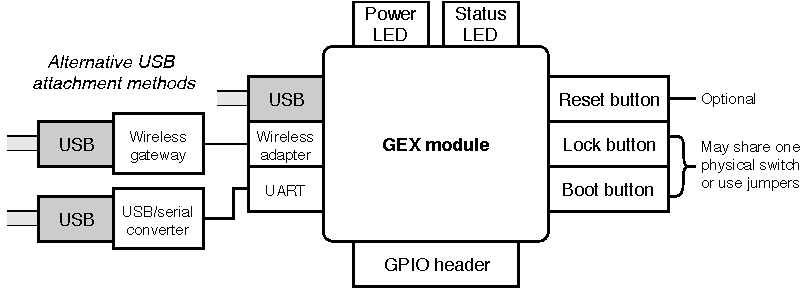
\includegraphics[scale=.95] {img/users-view.pdf}
	\caption{\label{fig:users-view-of-gex}Physical user interface of a GEX module}
\end{figure}

The GEX firmware can be flashed to a STM32 Nucleo or Discovery board or a custom \gls{PCB}. Discovery boards are equipped with a ``user \gls{USB}'' connector routed to the application \gls{MCU}; Nucleo boards have only the ST-Link \gls{USB} connector and, since the ST-Link version 2.1, offer a built-in USB-serial converter leading to one of the \gls{MCU}'s hardware \glspl{UART}.

After powering on, GEX loads its configuration from the Flash memory, configures its peripherals, sets up the function blocks and enables the selected communication interface(s). From this point, the module is operational and can be configured or used as needed by the user.

The physical user interface of the module is shown in figure \ref{fig:users-view-of-gex}. When a \gls{USB} cable connects the board to a \gls{PC}, the \gls{PC} \gls{OS} enumerates it and either recognizes the communication interface as \gls{CDCACM} (Virtual serial port), or leaves it without a software driver attached, to be accessed directly as raw \gls{USB} endpoints, based on GEX settings.
The connection using a physical UART and a USB/UART adapter works in a very similar way, as does the wireless connection (described in more detail below).

\subsection{Updating GEX Settings}

Two ways exist in which the module's settings can be modified: via the virtual Mass Storage disk, and through the control interface. We'll look at the file system method here; the API for a programmatic loading and updating of configuration will be explained in section \ref{sec:tf-bulk-rw}.

The board is equipped with a button or a jumper labeled Lock. When the button is pressed or the jumper removed (or inserted, the polarity is configured in the firmware), the Mass Storage \gls{USB} interface is enabled. For the user, this means that a new disk will appear on their computer which they can open in a file manager. The disk provides a read/write access to configuration files. 

The user edits a file as needed and saves it back to the disk. GEX processes the new content, tries to apply the changes and generates an updated version that includes any error messages or newly generated sections (when a new unit was registered). For the \gls{PC} \gls{OS} to recognize this change, the Mass Storage device momentarily reports that the media is unavailable to force the \gls{OS} to reload it. This is a similar mechanism to what happens when a memory card is removed from a reader. Now the user can reload the file in their editor, inspect the updated content and correct any possible mistakes. The settings, when applied successfully, should be immediately available to test using the communication interface. When everything is to the user's satisfaction, the updated settings are committed to the device's Flash memory by pressing the LOCK button again, or replacing the jumper.

\subsection{Connecting Using the Wireless Module}

In the case when a wireless module is installed on the \gls{PCB} and GEX is configured to use it, the radio link becomes a fallback connection when the \gls{USB} peripheral does not get enumerated within a short time after start-up.

To use it, the user needs to connect a wireless gateway module to their host \gls{PC} and use the radio link instead of a \gls{USB} cable. This connection works in a way similar to the hardware UART interface: it can be used to read and modify the configuration files and to access the functional blocks; the difference lies in a slightly different protocol required to communicate with the gateway itself, e.g. to pair it with the GEX module.

\subsection{Using the Control Interface}

Now that GEX is connected and configured, the user can start using it. This involves writing a program in C or Python that uses the GEX client library, using the Python library from MATLAB, or controlling GEX using a \gls{GUI} front-end built on those libraries. The configuration can be stored in the module, but it is also possible to temporarily replace it using the control \gls{API}. This way, the settings are loaded automatically when the user's program starts and may differ for different programs.

\section{Internal Structure Block Diagram}

The data flows and other internal logic of the firmware are depicted in figure \ref{fig:gex-internal}, with more explanation following in this chapter. The interchangeable role of the three communication interfaces can be clearly seen in the diagram, as well as the central role of the message queue which decouples interrupts from the processing thread.

\begin{figure}[h]
	\centering
	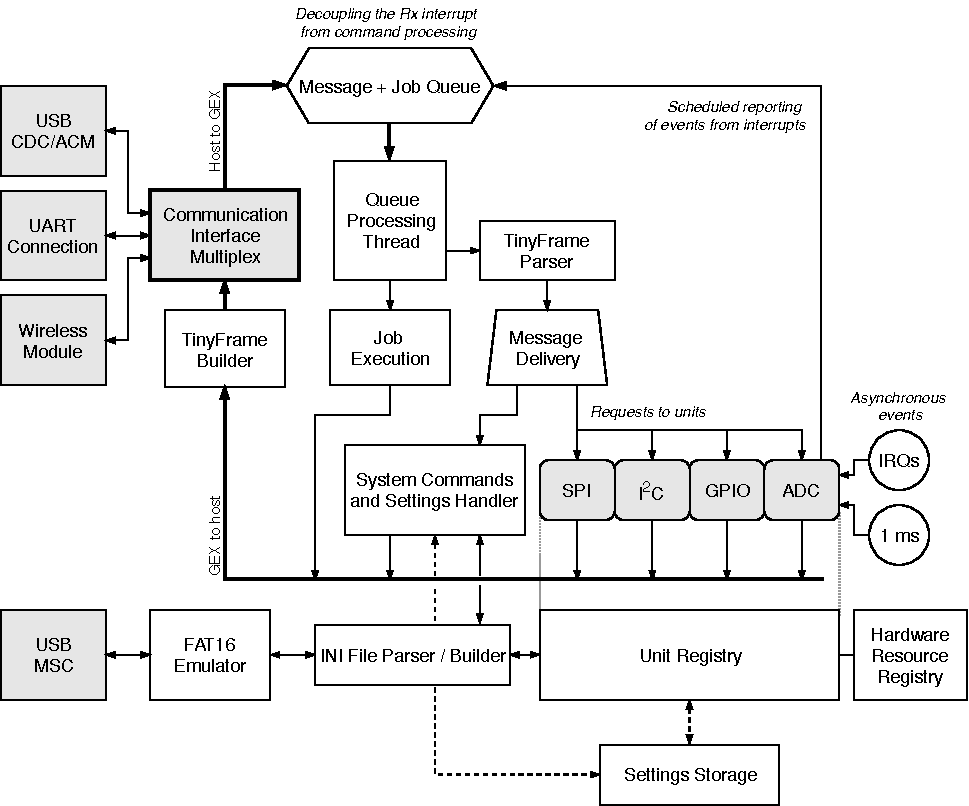
\includegraphics[scale=1] {img/gex-internal.pdf}
	\caption{\label{fig:gex-internal}Block diagram showing the internal logic in the GEX firmware}
\end{figure}

\section{FreeRTOS Synchronization Objects Usage}

The firmware is built on FreeRTOS (\ref{sec:freertos}) and a number of its synchronization objects and patterns are used to make its operation more robust.

\subsection{Message and Job Queue}

The message and job queue, seen in figure \ref{fig:gex-internal}, is used to decouple asynchronous interrupts from message transmission. All three communication interfaces use interrupts for the asynchronous handling of incoming messages. The same interrupt handler receives an event after a transmission was completed. The queue ensures that messages can be received during the transmission of a large response that demands the use of multiple transmissions.

The ``transmission complete'' interrupt signals this fact to the message processing task using a binary semaphore. The semaphore is released in the interrupt and take before a new block of data is transmitted. If more data needs to be transmitted, the queue task waits on the semaphore and enters a Blocked state until the semaphore becomes available again.

Two mutexes are used in the firmware: one that guards access to TinyFrame until the previous message was fully transmitted, and one to guard a shared memory buffer used, among other, by unit drivers during the serialization and parsing of a configuration file. The hardware resource registry (explained in \ref{sec:res-allocation}) does not need mutexes for individual resources, as a concurrent access to those fields can never happen thanks to the way the system is organized.

\section{Functional Blocks} \label{sec:units-function}

GEX's user-facing functions are implemented in \textit{unit drivers}. Those are mutually independent modules in the firmware that the user can enable and configure using a configuration file. There can be multiple instances of each unit type. However, we are limited by hardware constraints: e.g., there may be only one \gls{ADC} peripheral, two \gls{SPI} ports and so on. The assignment of those hardware resources to units is handled by the \textit{resource registry} (\ref{sec:res-allocation}).

Each unit is defined by a section in the configuration file \verb|UNITS.INI|. It is given a name and a \textit{callsign}, which is a number that serves as an address for message delivery. A unit is internally represented by a data object with the following structure:

\begin{itemize}
	\item Name
	\item Callsign (one byte)
	\item Configuration parameters loaded from the unit settings
	\item State variables updated at run-time by user commands or internal functions
	\item A reference to the unit driver
\end{itemize}

The unit driver handles commands sent from the host \gls{PC}, initializes and de-initializes the unit based on its settings, and implements other aspects of the unit's function, such as periodic updates and interrupt handling. Unit drivers may expose public \gls{API} functions to make it possible to control the unit from a different driver, allowing the creation of "macro units".

\section{Source Code Layout}

\begin{wrapfigure}[22]{r}{0.4\textwidth}
	\scriptsize\vspace{-3em}
	\begin{verbatim}
	├── build
	│   ├── firmware.bin
	│   └── firmware.dfu
	├── Drivers
	│   ├── CMSIS
	│   │   └── Device / ST / STM32F0xx
	│   └── STM32F0xx_HAL_Driver
	├── Middlewares / Third_Party / FreeRTOS
	├── Src
	│   └── main.c
	├── User
	│   ├── USB / STM32_USB_Device_Library
	│   │   ├── Class
	│   │   │   ├── CDC
	│   │   │   ├── MSC
	│   │   │   └── MSC_CDC
	│   │   └── Core
	│   ├── platform
	│   │   ├── plat_compat.h
	│   │   └── platform.c
	│   ├── units
	│   │   ├── adc
	│   │   ├── digital_out
	│   │   ...
	│   ├── FreeRTOSConfig.h
	│   └── gex.mk
	└── Makefile
	\end{verbatim}
	\vspace{-1em}
	\caption{\label{fig:repo-structure} The general structure of the source code repository}
\end{wrapfigure}

Looking at the source code repository (fig. \ref{fig:repo-structure}), at the root we'll find the device specific driver libraries and support files provided by ST Microelectronics, the FreeRTOS middleware, and a folder called \verb|User| containing the GEX application code. This division is useful when porting the firmware to a different microcontroller, as the GEX folder is mostly platform-independent and can be simply copied (of course, adjustments are needed to accompany different hardware peripheral versions etc.). The GEX core framework consists of everything in the \verb|User| folder, excluding the \verb|units| directory in which the individual units are implemented. Each unit driver must be registered in the file \verb|platform.c| to be available for the user to select. The file \verb|plat_compat.c| includes platform-specific headers and defines e.g. which pin to use for a status \gls{LED} or the LOCK button.

The \gls{USB} Device library, which had to be modified to support a composite class, is stored inside the \verb|User| folder too, as it is compatible with all STM32 microcontrollers that support \gls{USB}.


\section{Functions of the Core Framework}

The core framework forms the skeleton of the firmware and usually doesn't need any changes when new user-facing features are added. It provides the following services:

\begin{itemize}
	\item Hardware resource allocation (\ref{sec:res-allocation})
	\item Settings storage and loading (\ref{sec:settings-storage})
	\item Functional block (\textit{units}) initialization (\ref{sec:units-function})
	\item The communication port with different back-ends: \gls{USB}, \gls{UART}, wireless (\ref{sec:com-ports})
	\item Message sending and delivery (\ref{sec:message_passing})
	\item Interrupt management and routing to functional blocks (\ref{sec:irq-routing})
	\item Virtual mass storage for configuration file editing
\end{itemize}

When the firmware needs to be ported to a different STM32 microcontroller, the core framework is relatively straightforward to adapt and the whole process can be accomplished in a few hours. The time consuming part is modifying the functional blocks to work correctly with the new device's hardware.


\subsection{Resource Allocation} \label{sec:res-allocation}

\begin{figure}[h]
	\centering
	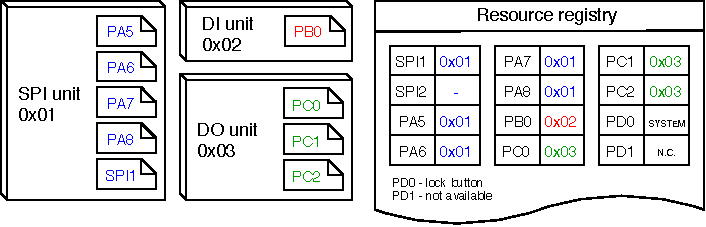
\includegraphics[scale=1] {img/resource-repository.pdf}
	\caption{\label{fig:resource-repository}An example allocation in the resource registry}
\end{figure}

The microcontroller provides a number of hardware resources that require exclusive access: GPIO pins, peripheral blocks (\gls{SPI}, \gls{I2C}, \gls{UART}\textellipsis), \gls{DMA} channels. If two units tried to control the same pin, the results would be unpredictable; similarly, with a multiple access to a serial port, the output would be a mix of the data streams and completely useless.

To prevent a multiple access, the firmware includes a \textit{resource registry} (fig. \ref{fig:resource-repository}). Each individual resource is represented by a field in a resource table together with its owner's callsign. Initially all resources are free, except for those not available on the particular platform (i.e. a GPIO pin PD1 may be disabled if not present on the microcontroller's package).

The resources used by the core framework are taken by a virtual unit \verb|SYSTEM| on start-up to prevent conflicts with the user's units. This is the case of the status \gls{LED}, the LOCK button, \gls{USB} pins, the communication \gls{UART}, the pins and an \gls{SPI} peripheral connecting the wireless module, pins used for the crystal oscillator, and the timer/counter which provides the system timebase.


\subsection{Settings Storage} \label{sec:settings-storage}

\begin{figure}[h]
	\centering
	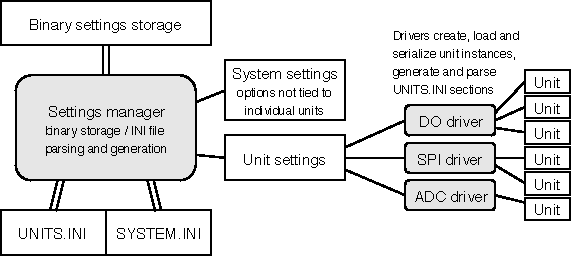
\includegraphics[scale=1] {img/settings-storage.pdf}
	\caption{\label{fig:settings-storage}Structure of the settings subsystem}
\end{figure}

The system and unit settings are written, in a binary form, into designated pages of the microcontroller's Flash memory. The unit settings serialization and parsing is implemented by the respective unit drivers.

As the settings persist after a firmware update, it is important to maintain backwards compatibility. This is achieved by prefixing the settings block of each unit with a version number. When the settings are loaded by a new version of the firmware, it first checks the version and decides whether to use the old or new format. When the settings are next changed, the new format will be used.

The INI files, which can be edited through the communication \gls{API} or using a text editor with the virtual mass storage, are parsed and generated on demand and are never stored in the Flash or \gls{RAM}, other than in short temporary buffers. The INI parser processes the byte stream on-the-fly as it is received, and a similar method is used to build a INI file from the configured units and system settings.

\subsection{Communication Ports} \label{sec:com-ports}

The firmware supports three different communication ports: hardware \gls{UART}, \gls{USB} (virtual serial port), and a wireless connection. Each interface is configured and accessed in a different way, but for the rest of the firmware (and for the \gls{PC}-side application) they all appear as a full duplex serial port. To use interfaces other than \gls{USB}, the user must configure those in the system settings (a file \verb|SYSTEM.INI| on the configuration disk).

At start-up, the firmware enables the \gls{USB} peripheral, configures the device library and waits for enumeration by the host \gls{PC}. When not enumerated, it concludes the \gls{USB} cable is not connected, and tries some other interface. The \gls{UART} interface cannot be tested as reliably, but it is possible to measure the voltage on the Rx pin. When idle, a \gls{UART} Rx line should be high (here 3.3\,V). The wireless module, when connected using \gls{SPI}, can be detected by reading a register with a known value and comparing those.

\subsubsection{USB Connection}

GEX uses vid:pid \verb|1209:4c60| and the wireless gateway \verb|1209:4c61|. The \gls{USB} interface uses the \gls{CDCACM} \gls{USB} class (\ref{sec:cdc-acm}) and consists of two bulk endpoints with a payload size of up to 64 bytes.

\subsubsection{Communication UART}

The parameters of the communication \gls{UART} (such as the baud rate) are defined in \verb|SYSTEM.INI|. It is mapped to pins PA2 and PA3; this is useful with STM32 Nucleo boards that do not include a User \gls{USB} connector, but provide a \gls{USB}-serial bridge using the on-board ST-Link programmer, connected to those pins.

This is identical to the \gls{USB} connection from the \gls{PC} application's side, except a physical \gls{UART} is necessarily slower and does not natively support flow control. The use of the Xon and Xoff software flow control is not practical with binary messages that could include those bytes by accident, and the ST-Link \gls{USB}-serial adapter does not implement hadware flow control.

\subsubsection{Wireless Connection}

The wireless connection uses an on-board communication module and a separate device, a wireless gateway, that connects to the \gls{PC}. The wireless gateway is interfaced differently from the GEX board itself, but it also shows as a virtual serial port on the host \gls{PC}. This is required to allow communicating with the gateway itself through the \gls{CDCACM} interface in addition to addressing the end devices.

This interface will be explained in more detail in chapter \ref{sec:wireless}.

\subsection{Message Passing} \label{sec:message_passing}

One of the key functions of the core framework is to deliver messages from the host \gls{PC} to the right units. This functionality resides above the framing protocol, which will be described in chapter \ref{sec:tinyframe}.

A message that is not a response in a multi-part session (this is handled by the framing library) is identified by its Type field. Two main groups of messages exist: \textit{system messages} and \textit{unit messages}. System messages can access the INI files, query a list of the available units, restart the module etc. Unit messages are addressed to a particular unit by their callsign (see \ref{sec:units-function}), and their payload format is defined by the unit driver. The framework reads the message type, then the callsign byte, and tries to find a matching unit in the unit list. If no unit with the callsign is found, an error response is sent back, otherwise the unit driver is given the message to handle it as required.

The framework provides one more messaging service to the units: event reporting. An asynchronous event, such as an external interrupt, an \gls{ADC} trigger or an \gls{UART} data reception needs to be reported to the host. This message is annotated by the unit callsign so the user application knows its origin.


\subsection{Interrupt Routing} \label{sec:irq-routing}

Interrupts are an important part of almost any embedded application. They provide a way to rapidly react to asynchronous external or internal events, temporarily leaving the main program, jumping to an interrupt handler routine, and then returning back after the event is handled. Interrupts are also the way FreeRTOS implements multitasking without a multi-core processor.

In the Cortex-M0-based STM32F072, used in the initial GEX prototypes, the interrupt handlers table, defining which routine is called for which interrupt, is stored in the program memory and cannot be changed at run-time. This is a complication for the modular structure of GEX where different unit drivers may use the same peripheral, and we would want to dynamically assign the interrupt handlers based on the active configuration. Let's have a look at an interrupt handler, in this case handling four different \gls{DMA} channels, as is common in STM32 microcontrollers:

\begin{minted}{c}
void DMA1_Channel4_5_6_7_IRQHandler(void)
{
    if (LL_DMA_IsActiveFlag_GI4(DMA1)) { /* handle DMA1 channel 4 */ }
    if (LL_DMA_IsActiveFlag_GI5(DMA1)) { /* handle DMA1 channel 5 */ }
    if (LL_DMA_IsActiveFlag_GI6(DMA1)) { /* handle DMA1 channel 6 */ }
    if (LL_DMA_IsActiveFlag_GI7(DMA1)) { /* handle DMA1 channel 7 */ }
}
\end{minted}

It is evident that multiple units might need to use the same interrupt handler, even at the same time, since each \gls{DMA} channel is configured, and works, independently. GEX implements a redirection scheme to accomplish such interrupt sharing: All interrupt handlers are defined in one place, accompanied by a table of function pointers. When a unit driver wants to register an interrupt handler, it stores a pointer to it in this redirection table. Then, once an interrupt is invoked, the common handler checks the corresponding entry in the table and calls the referenced routine, if any. Conversely, when a unit driver deinitializes a unit, it removes all interrupt handlers it used, freeing the redirection table slots for other use.











